%%%%%%%%%%%%%%%%%%%%%%%%%%%%%%%%%%%%%
% Document properties and packages
%%%%%%%%%%%%%%%%%%%%%%%%%%%%%%%%%%%%%
\documentclass[a4paper,11pt,final]{memoir}
\usepackage{CJKutf8}%中文支持

% misc
\renewcommand{\familydefault}{bch}	% font
\pagestyle{empty}					% no pagenumbering
\setlength{\parindent}{0pt}			% no paragraph indentation
% required packages (add your own)
\usepackage{flowfram}% column layou
\usepackage{marvosym}
\usepackage{textcomp}

\usepackage[top=1cm,left=1cm,right=1cm,bottom=1cm]{geometry}% margins
\usepackage{graphicx}										% figures
\usepackage{hyperref}
\definecolor{linkcolour}{rgb}{0,0.2,0.6}  %蓝色
\hypersetup{colorlinks,breaklinks,urlcolor=linkcolour, linkcolor=linkcolour}										% URLs
\usepackage[usenames,dvipsnames]{xcolor}					% color
\usepackage{multicol}										% columns env.
	\setlength{\multicolsep}{0pt}
\usepackage{paralist}										% compact lists
\usepackage{tikz}

%%%%%%%%%%%%%%%%%%%%%%%%%%%%%%%%%%%%%
% Create column layout
%%%%%%%%%%%%%%%%%%%%%%%%%%%%%%%%%%%%%
% define length commands
\setlength{\vcolumnsep}{\baselineskip}
\setlength{\columnsep}{\vcolumnsep}
%定义主题颜色,可选颜色 Maroon,ForestGreen,DarkOrchid,RoyalBlue,Turquoise,Cyan,etc,更多颜色参考xcolor包的颜色定义
\newcommand{\myThemeColor}{RoyalBlue}
% frame setup (flowfram package)
% left frame
\newflowframe{0.23\textwidth}{\textheight}{0pt}{0pt}[left]
	\newlength{\LeftMainSep}
	\setlength{\LeftMainSep}{0.23\textwidth}
	\addtolength{\LeftMainSep}{1\columnsep}
 
% small static frame for the vertical line
\newstaticframe{1.5pt}{\textheight}{\LeftMainSep}{0pt}
 
% content of the static frame
\begin{staticcontents}{1} %绘制分割线,使用tikz包绘制。如需改变风格线样式,请参考tikz教程,对于新手,不建议修改。
\hfill
\tikz{%
	\draw[loosely dotted,color=\myThemeColor,line width=1.5pt,yshift=0]
	(0,0) -- (0,\textheight);}%
\hfill\mbox{}
\end{staticcontents}
 
% right frame
\addtolength{\LeftMainSep}{1.5pt}
\addtolength{\LeftMainSep}{1\columnsep}
\newflowframe{0.7\textwidth}{\textheight}{\LeftMainSep}{0pt}[main01]


%%%%%%%%%%%%%%%%%%%%%%%%%%%%%%%%%%%%%
% define macros (for convience)
%%%%%%%%%%%%%%%%%%%%%%%%%%%%%%%%%%%%%
\newcommand{\Sep}{\vspace{1em}}
\newcommand{\SmallSep}{\vspace{0.9em}}

\newenvironment{AboutMe}
	{\ignorespaces\textbf{\color{\myThemeColor} About me}}
	{\Sep\ignorespacesafterend}
%定义section	
\newcommand{\CVSection}[1]
	{\Large\textbf{#1}\par
	\vspace{0.2cm}\normalsize\normalfont}

\newcommand{\CVItem}[1]
	{\textbf{\color{\myThemeColor} #1}}


%%%%%%%%%%%%%%%%%%%%%%%%%%%%%%%%%%%%%
% Begin document
%%%%%%%%%%%%%%%%%%%%%%%%%%%%%%%%%%%%%
\begin{document}

\begin{CJK*}{UTF8}{gbsn}%选择字体,黑体
% Left frame 左边内容在此定义
%%%%%%%%%%%%%%%%%%%%
\begin{figure}
	\hfill
	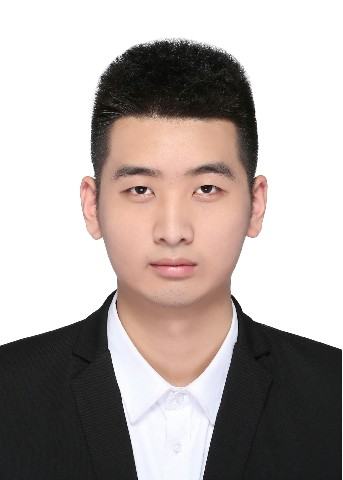
\includegraphics[width=0.8\columnwidth]{avatar1}
	\vspace{-7cm}
\end{figure}
\begin{flushright}\footnotesize
.\\
\vskip 7cm
    \raggedright
	\CVItem{{\large 个人信息:}}\\
	电子邮件:\\
	\href{mailto:yingpengma@gmail.com}{yingpengma@gmail.com}  \\
	个人主页:\\
	\href{https://ingingx.github.io/}{https://ingingx.github.io/}\footnote{该站仍在建设中} \\
	手机:\\
	+86 - 15108482982

	\CVItem{{\large 政治面貌:}}\\
	\textit{党员}

		
	\CVItem{{\large 语言能力:}}\\
	\textit{\textbf{英语}:\\
		    ~~TOEFL iBT: 83/120\\
		    ~~GRE: 319+3.0/340\\
		    ~~四级、六级:通过\\
		   \textbf{中文}:母语 \\ 
		   \textbf{德语}:简单沟通
			}
	
	\CVItem{{\large 电脑技能:}}\\
	$\bullet$\textbf{编程语言:}\\ C/C++/MATLAB/Python 以及 Java, HTML5等 \\
	$\bullet$\textbf{工作软件:}\\ Excel/PowerPoint/Word, PS, 以及 AfterEffect等 \\
	$\bullet$\textbf{科学计算:}\\ MATLAB \\
	\SmallSep
	\textit{熟练使用\LaTeX \footnote{本简历使用\LaTeX编辑制作} 和LINUX,能够在Android平台上编写简单的App}

	\CVItem{{\large 我与微臣:}}\\
	\textit{在2016年开始准备语言时就关注了微臣,之后由于家里经济条件和课程太忙,并没有上课(遗憾啊).在微臣公众号(@微臣留美 @臣在托福)里收获了许多关于托福,GRE的知识和tips.虽然之前备考没有听过微臣老师讲课,但是依然希望领略老师们的风采,这也是申请成为助教的原因之一.虽然我的成绩并不十分出色,但是我与托福,GRE,ETS爸爸纠葛十分之深 \footnote{考过5次TOEFL,历时一年半。最近一次18年11月,本想100+,却被“制裁”:non-scorable} ,自认为备考经验比较丰富.也因托福没上百,GRE没325+感到遗憾.希望下次托福100+,大概是申请助教的原因之二吧}
	\SmallSep
\end{flushright}\normalsize
\framebreak


% Right frame 右边内容在此定义
%%%%%%%%%%%%%%%%%%%%%
\Huge\bfseries {\color{\myThemeColor} 马~瀛~鹏~~Ma, Yingpeng}\\
\normalsize\normalfont

% Education
\CVSection{教育背景 \footnote{已经收到南卡罗来纳大学 (SC) CE全奖Ph.D. offer}}
\hrule
\SmallSep
\CVItem{2015.09 - 目前\hfill\textsc{电子科技大学~UESTC,四川成都}}\\
\textit{-信息与通信工程学院}\\
\textit{-通信工程}
\\
\CVItem{2016.08 - 2016.09\hfill\textsc{新加坡国立大学~NUS,新加坡}}\\
\textit{-暑假课程}
\\
\CVItem{2012.09 - 2015.06\hfill\textsc{西北师范大学附属中学~HSANNU,甘肃兰州}}\\
\textit{-高中理科班}
\\


% Experience
\CVSection{实习经历}
\hrule
\SmallSep
\CVItem{2017.08 - 2017.09 \hfill 大唐电信,成都}\\
\textit{$\bullet$ 实习研究助理,辅助搭建与初始化电信基站,研究最佳分配算法并仿真}
\\
\CVItem{2016.09 - 2016.10 \hfill 创青春大赛,电子科技大学}\\
\textit{$\bullet$ 担任志愿者,指引参赛学生出入场,维护赛场秩序}
\\
\CVItem{2016.08 - 2016.09 \hfill ERA,新加坡}\\
\textit{$\bullet$ 市场调查,调研新加坡市场对房地产的价格需求,并获优秀实习生推荐信} 
\\
\CVItem{2015.09 - 2015.12\hfill Syslab,电子科技大学}\\
\textit{$\bullet$ 实习开发员,与组员一同完成了简单app的构思、设计、开发全流程}
\\
\CVItem{2015.09 - 2016.06\hfill 通信学院学生会,电子科技大学}\\
\textit{$\bullet$ 担任“新青年”部员,策划、组织、参与“荧光夜跑”、“迎新晚会”等多场活动}
\\
\CVItem{2015.09 - 2016.06\hfill 班长,电子科技大学}\\
\textit{$\bullet$ 负责班级建设、管理、活动组织等多项事务,与同学建立良好友谊}
\\

% CAMPU
\CVSection{专业经历}
\hrule
\SmallSep
\CVItem{2017.9 - 目前,基于Bitmap的显著性探索\hfill\emph{}研究员}\\
\textit{$\bullet$ 分析图像Bitmap以及编码信息,作为预处理步骤,尝试改进已有显著性检测方案。目前团队力图改进该方案,使之可以作为绝大多数已有显著性检测模型的增强方法} 
\\
\CVItem{2017.12 - 2018.03, 基于 Bitplane Slicing 的显著性检测\hfill\emph{团队领导}}\\
\textit{$\bullet$ 分析图像Bitplane Slicing信息,总结可利用内容,构建脱离深度学习框架的图片显著性检测模型,并在大量数据集上测试,对比先进模型,提出不足与改进方案。该项目参与“2018年大学生创新创业项目”,完成答辩,并获“\textbf{通过}”评价} 
\\
\CVItem{2018.05 - 2018.07, SIMO系统性能仿真分析 \hfill\emph{团队领导}}\\
\textit{$\bullet$ 学习了解SIMO技术,利用MATLAB与SIMILINK对其仿真,撰写实验报告,获老师好评} 
\\
\CVItem{2017.12 - 2018.01, H.265视频编码技术综述 \hfill\emph{研究员}}\\
\textit{$\bullet$ 深入了解H。265先进视频编码技术,与其他编码技术对比性能,总结成文,获A级评价} 
\\
\CVItem{2017.11 - 2017.12, 基于AUX的信息传输\hfill\emph{团队领导}}\\
\textit{$\bullet$ 利用AUX音频传输线,设计调制解调模块与编码方案,在两台电脑之间实现图片、音频、文字的实时传输}
\\

% HONORS & SCHOLARSHIPS
\CVSection{个人荣誉}
\hrule
\SmallSep
	\begin{tabular}{l|l}
		$\Rightarrow$ 2016&\textit{电子科技大学社会实践优秀个人}\footnotesize\\
		$\Rightarrow$ 2016&\textit{电子科技大学数学竞赛三等奖}\\
	\end{tabular}

%%%%%%%%%%%%%%%%%%%%%%%%%%%%%%%%%%%%%
% End document
%%%%%%%%%%%%%%%%%%%%%%%%%%%%%%%%%%%%%
\end{CJK*}
\end{document}